\documentclass[tikz, border=5mm]{standalone}
\usetikzlibrary{positioning, arrows.meta, calc, fit, backgrounds, shapes.geometric, patterns, decorations.pathreplacing}

\begin{document}
	
	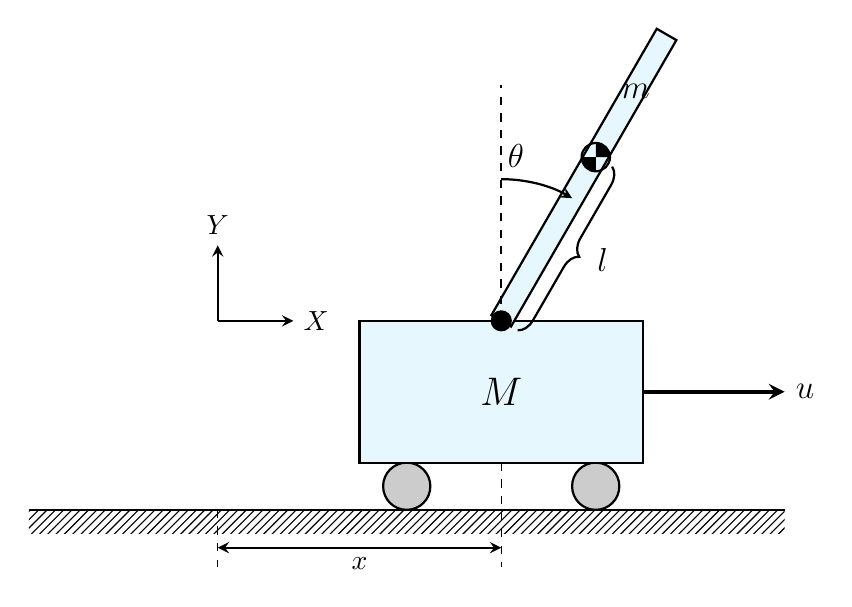
\begin{tikzpicture}[>=stealth, scale=1.2]
		
		% Definición de parámetros para dibujar (puedes cambiarlos a tu gusto)
		\def\W{3}       % Ancho del carro
		\def\H{1.5}     % Alto del carro
		\def\x{3}       % Posición actual x del carro
		\def\L{2}       % Longitud del péndulo al CM
		\def\Ltotal{3.5}  % Longitud física de la barra (mayor que \L)
		\def\ang{30}    % Ángulo theta en grados
		\def\Rrueda{0.25} % Radio de las ruedas
		
		% --- 1. SUELO Y REFERENCIA FIJA ---
		\draw[thick] (-2, 0) -- (6, 0);
		\fill[pattern=north east lines] (-2, -0.25) rectangle (6, 0);
		
		% Origen de coordenadas fijo (x=0)
		\draw[->, thick] (0, 2) -- (0.8, 2) node[right] {$X$};
		\draw[->, thick] (0, 2) -- (0, 2.8) node[above] {$Y$};
		
		% --- 2. EL CARRO ---
		\coordinate (CentroCarro) at (\x, \Rrueda);
		
		% Ruedas
		\draw[thick, fill=gray!40] (\x - \W/2 + 0.5, \Rrueda) circle (\Rrueda);
		\draw[thick, fill=gray!40] (\x + \W/2 - 0.5, \Rrueda) circle (\Rrueda);
		
		% Cuerpo del carro
		\draw[thick, fill=cyan!10] (\x - \W/2, 2*\Rrueda) rectangle (\x + \W/2, 2*\Rrueda + \H);
		\node at (\x, 2*\Rrueda + \H/2) {\Large $M$};
		
		% Cota de la posición x
		\draw[dashed] (\x, 2*\Rrueda) -- (\x, -0.6);
		\draw[dashed] (0, 0) -- (0, -0.6);
		\draw[<->, thick] (0, -0.4) -- (\x, -0.4) node[midway, below] {$x$};
		
		% Fuerza u (Acción de control)
		\draw[->, line width=1.5pt] (\x + \W/2, 2*\Rrueda + \H/2) -- ++(1.5, 0) node[right] {\large $u$};
		
		% --- 3. EL PÉNDULO ---
		% Pivote
		\coordinate (Pivote) at (\x, 2*\Rrueda + \H);
		
		% Centro de Masas (CM) usando trigonometría básica
		\coordinate (CM) at ({\x + \L*sin(\ang)}, {2*\Rrueda + \H + \L*cos(\ang)});
		
		% Barra del péndulo
		% Definir el extremo físico de la barra
		\coordinate (Extremo) at ({\x + \Ltotal*sin(\ang)}, {2*\Rrueda + \H + \Ltotal*cos(\ang)});
		
		% Barra del péndulo con contorno y relleno igual al carro
		\draw[thick, fill=cyan!10, rotate around={-\ang:(Pivote)}] (\x-0.12, 2*\Rrueda + \H) rectangle (\x+0.12, 2*\Rrueda + \H + \Ltotal);
		
		% Eje central del pivote
		\draw[thick, fill=black] (Pivote) circle (0.1);
		
		% Punto del Centro de Masas
		\begin{scope}[shift={(CM)}]
			\fill[black] (0,0) -- ++(0.15,0) arc (0:90:0.15) -- cycle;
			\fill[black] (0,0) -- ++(-0.15,0) arc (180:270:0.15) -- cycle;
			\draw[thick] (0,0) circle (0.15);
			\node[right=0.2cm] at (0,0.7) {\large $m$};
		\end{scope}
		
		% --- 4. ÁNGULOS Y LONGITUDES ---
		% Línea vertical discontinua
		\draw[dashed, thick] (Pivote) -- ++(0, \L + 0.5) coordinate (Top);
		
		% Arco del ángulo theta
		\draw[->, thick] (\x, 2*\Rrueda + \H + 1.5) arc[start angle=90, end angle={90-\ang}, radius=1.5];
		\node at ({\x + 0.6*sin(\ang/2)}, {2*\Rrueda + \H + 1.5*cos(\ang/2) + 0.3}) {\large $\theta$};
		
		% Llave para indicar la longitud l al CM
		\draw[decorate,decoration={brace,amplitude=6pt,mirror}, thick]
		($(Pivote)!0.2cm!-90:(CM)$) -- ($(CM)!0.2cm!90:(Pivote)$) node[midway, right=8pt, yshift=-4pt] {\large $l$};
		
	\end{tikzpicture}
	
\end{document}